\documentclass[12pt]{article}
 
\usepackage[margin=1in]{}
\usepackage{amsmath,amsthm,amssymb,graphicx,geometry,mathtools,tikz,hyperref,outlines}

\usetikzlibrary{positioning}

\renewcommand{\d}[1]{\ensuremath{\operatorname{d}\!{#1}}}
\newcommand{\n}{\mathbb{N}}
\newcommand{\z}{\mathbb{Z}}
\newcommand{\q}{\mathbb{Q}}
\newcommand{\cx}{\mathbb{C}}
\newcommand{\real}{\mathbb{R}}
\newcommand{\field}{\mathbb{F}}
\newcommand{\ita}[1]{\textit{#1}}
\newcommand{\com}[2]{#1\backslash#2}
\newcommand{\oneton}{\{1,2,3,...,n\}}
\newcommand\idea[1]{\begin{gather*}#1\end{gather*}}
\newcommand\ef{\ita{f} }
\newcommand\eff{\ita{f}}
\newcommand\proofs[1]{\begin{proof}#1\end{proof}}
\newcommand\inv[1]{#1^{-1}}
\newcommand\setb[1]{\{#1\}}
\newcommand\en{\ita{n }}
\newcommand{\vbrack}[1]{\langle #1\rangle}
\newcommand\Inn{\mathrel{\ooalign{$\subset$\cr\hfil\scalebox{0.8}[1]{$=$}\hfil\cr}}}

% https://tex.stackexchange.com/questions/32160/new-line-after-paragraph
\newcommand{\paragraphNewLine}[1]{\paragraph{#1}\mbox{}\\}

\def\Plus{\texttt{+}}
\def\Minus{\texttt{-}}


\newenvironment{theorem}[2][Theorem]{\begin{trivlist}
\item[\hskip \labelsep {\bfseries #1}\hskip \labelsep {\bfseries #2.}]}{\end{trivlist}}
\newenvironment{lemma}[2][Lemma]{\begin{trivlist}
\item[\hskip \labelsep {\bfseries #1}\hskip \labelsep {\bfseries #2.}]}{\end{trivlist}}
\newenvironment{exercise}[2][Exercise]{\begin{trivlist}
\item[\hskip \labelsep {\bfseries #1}\hskip \labelsep {\bfseries #2.}]}{\end{trivlist}}
\newenvironment{reflection}[2][Reflection]{\begin{trivlist}
\item[\hskip \labelsep {\bfseries #1}\hskip \labelsep {\bfseries #2.}]}{\end{trivlist}}
\newenvironment{proposition}[2][Proposition]{\begin{trivlist}
\item[\hskip \labelsep {\bfseries #1}\hskip \labelsep {\bfseries #2.}]}{\end{trivlist}}
\newenvironment{corollary}[2][Corollary]{\begin{trivlist}
\item[\hskip \labelsep {\bfseries #1}\hskip \labelsep {\bfseries #2.}]}{\end{trivlist}}
 \hypersetup{
 colorlinks,
 linkcolor=blue
 }
\begin{document}

 
\title{Math 221 Notes}
\author{VOGEL, Max}
\date{UW-Madison, Summer 2020}

% https://tex.stackexchange.com/questions/186981/is-there-a-subsubsubsection-command
\setcounter{tocdepth}{4}
\setcounter{secnumdepth}{4}

\maketitle
\tableofcontents
\newpage

\section{Week 1}
\subsection{Day 1}
\subsubsection{Factoring:}
$$(a+b)(a^2-ab+b^2)=a^3+b^3 $$
$$(a-b)(a^2+ab+b^2)=a^3-b^3 $$


\subsubsection{Rules:}
\begin{minipage}{0.45\textwidth}
$$ a < b \rightarrow{} -a > -b $$
$$ -ax < b \rightarrow{} x > -\frac{b}{a} $$
$$ |x| = b \rightarrow{} x = b \vee x = -b $$
$$ |x| < b \rightarrow{} -b < x < b $$
$$ |x| = b \rightarrow{} x > b \vee x < -b $$
$$ a^m a^n = a^{m+n} $$
$$ \frac{a^m}{a^n} = a^{m-n}$$
$$ (ab)^m=a^m b^m$$
\hfill
\end{minipage}
\begin{minipage}{0.45\textwidth}
\begin{tabular}{|p{\textwidth}}
$$ \left(\frac{a}{b}\right)^n = \frac{a^n}{b^n}$$
$$ (a^m)^n = a^{mn}$$
$$ \sqrt{a} = a^{\frac{1}{2}}$$
$$ \sqrt[n]{a} = a^{\frac{1}{n}}$$
$$ \left(\sqrt[n]{a}\right)^m = \sqrt[n]{a^m} = a^{\frac{m}{n}}$$
$$ \sqrt{a}\sqrt{b} = \sqrt{ab}$$
$$ \sqrt[n]{a} \sqrt[n]{b} = \sqrt[n]{ab}$$\\
\end{tabular}
\end{minipage}

\subsubsection{Functions:}

\textbf{Definition: }
Assigns each element $x$ in a set $D$ exactly one element, called $f(x)$, in set $E$.\\
In terms of a graph, a curve can only be a function if no vertical lines intersect the curve more than once (vertical line test).
\begin{itemize}
    \item The set $D$ is called the domain -- possible $x$ values.
    \item The set $E$ is called the range -- possible $y$ values.
    \item If $f$ is a function with domain $D$, then it graph is the set of ordered pairs\\
    $ \{(x, f(x) | x) \text{ is a element of, } \in{}, D\}$
\end{itemize}
\paragraph{Finding domain:}
\begin{enumerate}
    \item $f(x) = \sqrt{x+2}$
    $\rightarrow{} x + 2 \geq{} 0$
    $\rightarrow{} x \geq{} -2 $
    $\rightarrow{} [-2, +\infty)$
    
    \item $f(x) = \frac{1}{x^2-x} $
    $\rightarrow{} x^2-x \neq{} 0 $
    $\rightarrow{} x(x-1) \neq{} 0 $
    $\rightarrow{} x \neq{} 0 \wedge x \neq 1 $
    $\rightarrow{} (-\infty, 0) \cup (0, 1) \cup (1, +\infty)$
\end{enumerate}

\paragraph{Picewise:}
\begin{itemize}
    \item Open circles, $\circ$, and circle brackets, ( ), are non-inclusive.
    \item Closed circles, $\bullet$, and square brackets, [ ], are inclusive.
    \item Formatted as: 
    \item[] $f(x)=\begin{cases} 
              y=5   : x < 0 \\
              y=x^2 : x\geq 0 
            \end{cases}$
\end{itemize}

\paragraph{Types}
\begin{itemize}
    \item[] \textbf{Even: }
    \item A function is even if $f(x) = f(-x)$
    \item The graph is symmetric with respect to the y-axis.
    \item Examples: $x^4 - 2, x^{20}+x^6, \cos(x), |x|$

\end{itemize}

\begin{itemize}
    \item[] \textbf{Odd: }
    \item A function is even if $f(x) = -f(x)$
    \item The graph has rotational symmetry about origin.
    \item Examples: $x^3, x^{7}+x, \sin(x), |x|x$
\end{itemize}

\noindent\hrulefill

\begin{itemize}
    \item[-] Even times odd function is always odd.
    \item[-] Even times even is always even.
    \item[-] Odd times odd is always even.
\end{itemize}

\paragraphNewLine{Increasing \& Decreasing:}

\textbf{Increasing : } A  function $f$ is called increasing on an interval if $f(x_1) < f(x_2)$ whenever $x_1 < x_2$. In other words, the slope must always be positive.

\textbf{Decreasing : } A  function $f$ is called increasing on an interval if $f(x_1) > f(x_2)$ whenever $x_1 < x_2$. In other words, the slope must always be negative.


\subsubsection{Limits}

\textbf{Definition: } Supposing $f(x)$ is defined when $x$ is near the number $a$, we write $\lim_{x\to a} f(x) = L$ and say ``the limit of $f(x)$, as $x$ approaches $a$, equals $L$''.


\begin{itemize}
    \item $\lim_{x\to a} f(x) = L$ if and only if (iff, $\iff$) $\lim_{x\to a^-} f(x) = L \wedge \lim_{x\to a^+} f(x) = L$
    \item That is, the limit does not exist, $\nexists$, if $x$ approaches different values when from the left and right sides 
    \item Approaching from left (from $-\infty \to \infty$) is notated as $x \to a^-$
    \item Approaching from right (from $\infty \to -\infty$)) is notated as $x \to a^+$
    \item iff, $\iff$:
        $$A \iff B \rightarrow{}$$
        $$A \text{ is necessary and sufficient for B }\rightarrow{}$$
        $$B \text{ is necessary and sufficient for A } \rightarrow{}$$
        $$A \text{ is equivalent to } B$$
    \item A vertical asymptote exists if the limit from left side is $+\infty$ or $-\infty$, and the limit from the right side is the opposite.
\end{itemize}

\paragraph{Infinite Limits}
\begin{itemize}
    \item If function limit is $\pm \infty$ (if the denominator is 0 at $f(a)$), you can find whether its $\Plus{}$ or $\Minus{}$ by solving the limit for each term. If the term is positive, then it's $+ \infty$, and vice-versa, e.g.
    
    $$\lim_{x \to -2^+} \frac{x-1}{x^2(x+2)}$$
    $$\frac{\lim_{x \to -2^+} [x-1]}{ (\lim_{x \to -2^+} [x])^2 \cdot \lim_{x \to -2^+} [(x+2)]}$$
    $$\frac{\ominus}{\oplus \cdot \oplus}$$
    $$\ominus \rightarrow{} -\infty$$

\end{itemize}

\subsubsection{Lines}
\begin{itemize}
    \item Slope-Point form: $y-b = m(x+a)$ -- $(a,b)$ will be a point of the equation.
    \item Slope-Intercept form: $y = mx + b$ -- $(0,b)$ will be the $y$-intercept.
    \item Vertex form: $y = a(x-h)+k$ -- $(h,k)$ will be the vertex.
    \item Point-Point form: $y-y_1=\frac{y_2-y_1}{x_2-x_1}(x-x_1)$ -- $(x_1,y_1)$ and $(x_2,y_2)$ will be points of the equation.
    \item Intercept form:  $\frac{x}{a} + \frac{y}{b} = 1$  -- $(a, b)$ will be a point of the equation.
    
\end{itemize}

\subsection{Day 2}
\subsubsection{Limit Laws:}
Supposing $c$ is a constant and $\lim_{x \to a}f(x)$ and $\lim_{x \to a}g(x)$ exists, then\\
\begin{minipage}{0.5\textwidth}
    $$\lim_{x \to a} [f(x) \pm g(x)] = \lim_{x \to a} f(x) \pm \lim_{x \to a} g(x)$$
    $$\lim_{x \to a} [cf(x)] = c \cdot \lim_{x \to a} f(x)$$
    $$\lim_{x \to a} [f(x)g(x)] = \lim_{x \to a} f(x) \lim_{x \to a} g(x)$$
    $$\lim_{x \to a} \left [ \frac{f(x)}{g(x)} \right ] = \frac{\lim f(x)}{\lim g(x)} \text{ if } \lim_{x \to a} g(x) \neq{} 0$$
    $$\lim_{x \to a} [f(x)]^n = [\lim_{x \to a} f(x)]^n$$

\hfill
\end{minipage}
\begin{minipage}{0.45\textwidth}
\begin{tabular}{|p{\textwidth}}
$$\lim_{x \to a} c = c$$
$$\lim_{x \to a} x = a$$
$$\lim_{x \to a} x^n = a^n \text{ where } n = \mathbb{Z}^+$$ 
$$\lim_{x \to a} \sqrt[n]{x} = \sqrt[n]{a} \text{ where } n = \mathbb{Z}^+$$ 
$$\lim_{x \to a} \sqrt[n]{f(x)} = \sqrt[n]{f(a)} \text{ if } f(a) \geq 0 \text{ and } n_{even}$$
\end{tabular}
\end{minipage}

\noindent\textbf{Direct Substitution Property:} If $f$ is a polynomial or rational function, and $a$ is in the domain of $f$, then $\lim_{x \to a} f(x) = f(a)$\\
\textbf{Theorem 1.6.1:} If $f(x) = g(x)$ when $x \neq a$, then $\lim_{x\to a} f(x) = \lim_{x\to a} g(x)$ \\
\textbf{Theorem 1.5.1:} If $f(x) = L \iff \lim_{x\to a^-} f(x) = L = \lim_{x\to a^+} f(x)$\\
\textbf{Theorem 1.6.2:} If $f(x) \leq g(x)$ when $x$ is near $a$ and the limits of $f$ and $g$ both exist as $x$ approaches $a$, then $\lim_{x\to a} f(x) \leq \lim_{x\to a} g(x)$\\
\textbf{Squeeze Theorem:} If $f(x) \leq g(x) \leq h(x)$ when $x$ is near $a$ and 
 $\lim_{x\to a} f(x) =  \lim_{x\to a} h(x) = L$, then $\lim_{x\to a} g(x) = L$


\subsubsection{Piecewise / $(\epsilon, \delta)$ definition  of limit}
If for every small number $\epsilon >  0$ there is a number $\delta > 0$ such that if $0 < |x-c| < \delta$ then $|f(x) - L| < \epsilon$.

$$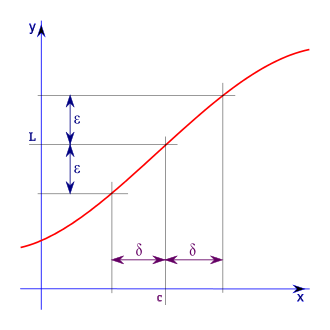
\includegraphics[scale=.5]{media/limit01.png}$$

\noindent Solving for $\delta$, rewrite the term defining $\epsilon$ to be equal to the term defining $\delta$. E.g., solving for $\delta$ if $|x-2|<\delta$, then $|4x-8|<\epsilon$, where $\epsilon = 0.1$:

$$|4x-8|=4|x-2|<0.1$$
$$|x-2| < \frac{0.1}{4}\text{, therefore } \delta=\frac{0.1}{4}$$

\noindent For non-linear equations, find the lesser and greater $\delta$, and choose the one that results in the smaller $\epsilon$.

\subsection{Day 3}
\subsubsection{Continuous Function:}
\textbf{Definition:} A function $f$ is continuous at  a number if $\lim_{x\to a} f(x) = f(a)$. Graphically, a function is continuous if you can draw it without having your pen leave paper. More formally, $f(x)$ is continuous at $x=a \iff:$ 

\begin{enumerate}
    \item $f(a)$ is defined ($a \in{} D: $ $a$ is in the domain of $f$).
    \item $\lim_{x\to a} f(x)$ exists, and equals $f(x) = f(a)$.
\end{enumerate}

If one of the aforementioned statements is incorrect, then $f(x)$ is discontinuous at $x=a$

\textbf{Theorem 1:} A function is continuous on an interval if it's continuous at every number in the interval. That is, if $f$ and $g$ are continuous at $x=a$, then the following are also continuous at $a$:\\
$$f+g, f-g, cf, fg, \frac{f}{g} \text{ for } g(a) \neq{} 0$$


\textbf{Theorem 2:} The following types of functions are continuous at every number in there domain: Polynomials, Rational functions, Root functions, \& Trig functions.\\


\textbf{Theorem 3: Intermediate Value Theorem (IVM):} Suppose that $f$ is continuous on the close interval $[a,b]$ and let $N$ be any number between $f(a)$ and $f(b)$, where $f(a) \neq{} f(b)$. Then there exists at least on number $c$ in $(a,b)$ such that $f(c)=N$. 

$$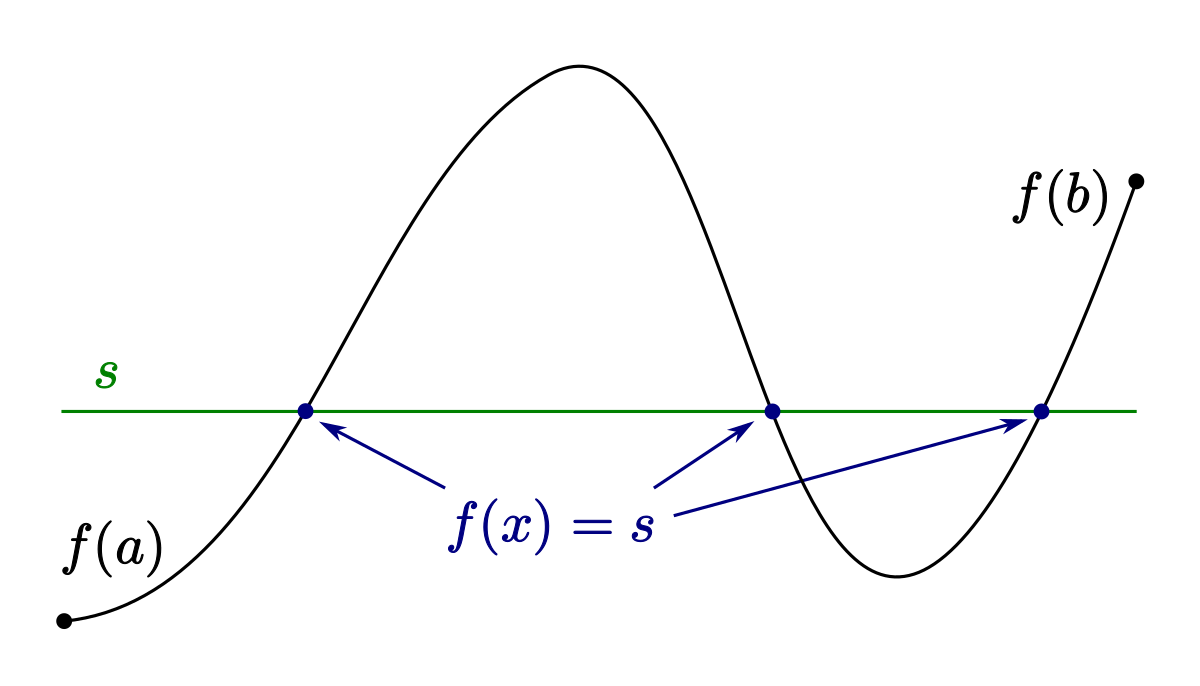
\includegraphics[scale=.2]{media/ivm.png}$$

\subsection{Day 4}
\subsubsection{Lines:}
\paragraph{Secant Line:} A line that locally intersects two points on a curve.

$$\frac{\text{Rise}}{\text{Run}} = \frac{\Delta y}{\Delta x} = \frac{y_1 - y_0}{x_1 - x_0} =  \frac{f(a+h)-f(a)}{(a+h)-a}=\frac{f(a+h)-f(a)}{h}$$

$$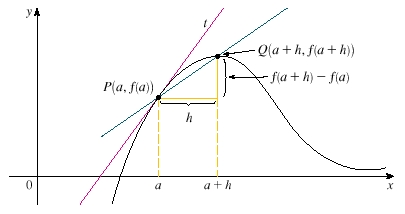
\includegraphics[scale=.5]{media/secanteq.jpg}$$

\paragraph{Tangent Line:} The line through a pair of infinitely close points on the curve so that the line is ``just touching''. Slope equation (also known as ``Difference Quotient''):

$$\lim_{h \to 0} \left [ \frac{f(a+h)-f(a)}{h} \right ]$$

\subsubsection{Derivatives:} The derivative of a function $f$ at a number $a$, denoted by $f'(a)$, is 

$$f'(a) = \lim_{h \to 0} \left [ \frac{f(a+h)-f(a)}{h} \right ]$$
and the equation of the tangent line to the curve $y=f(x)$ at the point $(a,f(a))$ can be written in point-slope form as

$$y-f(a)=f'(a)(x-a)$$

\subsection{Day 5}
\subsubsection{Derivatives (cont.):}
\begin{itemize}
    \item Other notation is $\frac{d y}{d x} |_{x=a}$ (Leibniz Notation),  $\frac{d f}{d x}$, $\frac{d}{d x}$ $f(x)$, $f(x)$, $D f(x)$, \& $D_{x} f(x)$
    \item Function $f(x)$ is differentiable at $x=a$ if $f'(a)$ exists (same as Theorem 1.5.1).
    \item Therefore, Not Continuous $\implies$ Not Differentiable.
    \item If $f'(a)$ exists, then $\lim_{x \to a} f(x) = f(a)$
    \item The derivative is a function, not a constant.
    \item Because $f'$ is also a function, $f'$ may have a derivative of its own, denoted by $(f')' = f''$ and called the \textbf{second derivative} of $f$. This can also be written as $\frac{d}{d x} \left ( \frac{d y}{d x} \right ) = \frac{d^2 y}{dx^2}$
\end{itemize}


\subsection{Day 6}
\subsubsection{Derivatives Rules:}

\begin{minipage}{0.5\textwidth}

\begin{itemize}
    \item Constant: $\frac{d}{d x}(c) = 0$
    \item Linear: $\frac{d}{d x}(x) = 1$
\end{itemize}

\end{minipage}
\begin{minipage}{0.45\textwidth}
\begin{tabular}{|p{\textwidth}}
\begin{itemize}
    \item Linear + Constant: $\frac{d}{d x}(ax) = a$
    \item Power Rule: $\frac{d}{d x}(x^n) = n x^{n-1}$
\end{itemize}
\end{tabular}
\end{minipage}

\begin{itemize}
    \item Constant Multiple: $\frac{d}{d x}[c \cdot f(x)] = c \cdot \frac{d}{d x}(f(x))$
    \item Sum/Difference: $\frac{d}{d x}[f(x) \pm g(x)] = f'\pm g'$
    \item Product Rule: $\frac{d}{d x}[f(x)\cdot g(x)] = f'\cdot g + f \cdot g'$
    \item Quotient Rule: $\frac{d}{d x}\left[ \frac{f(x)}{g(x)} \right] = \frac{g\cdot f'- f\cdot g'}{g^2} = \frac{\text{lo} \cdot \text{d hi - hi} \cdot \text{d lo}}{\text{lo}\cdot\text{lo}}$
\end{itemize}

\subsubsection{Lines:}
\textbf{Theorem:} If the graph of $y=m_1x+b_1$ is perpendicular to the graph of $y=m_2x+b_2$, then $m_1m_2 = -1$. 
\\
\textbf{Normal Line:} The normal line to a curve at point $M$ is the line through $M$ that is perpendicular to the tangent line at $M$.

$$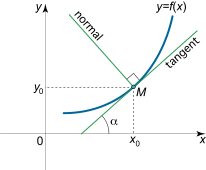
\includegraphics[scale=.8]{media/normal-tangent.png}$$


\subsection{Day 7}
\subsubsection{Trig Review:}
$$\csc = \frac{1}{\sin}, \ \sec = \frac{1}{\cos}, \ \cot = \frac{1}{\tan} = \frac{\cos}{\sin}$$
\subsubsection{Trig Identities:}
$$\sin^2 + \cos^2 = 1$$
$$\text{Dividing by }\sin^2: 1 + \frac{\cos^2}{\sin^2} = \frac{1}{\sin^2} \rightarrow{} 1 + \cot^2 = \csc^2$$
$$\text{Dividing by }\cos^2: \frac{\sin^2}{\cos^2} + 1 = \frac{1}{\cos^2} \rightarrow{} \tan^2 + 1 = \sec^2$$
\subsubsection{Derivative of Trig Functions:}
\begin{minipage}{0.5\textwidth}
    
    $$(\sin)' = \cos$$
    $$(\cos)' = -\sin$$
    $$(\tan)' = \sec^2 $$
\hfil
\end{minipage}
\begin{minipage}{0.45\textwidth}
\begin{tabular}{|p{\textwidth}}

    $$(\csc)' = -\cot \cdot \csc$$
    $$(\sec)' = \sec \cdot \tan$$
    $$(\cot)' = -\csc^2 $$

\end{tabular}
\end{minipage}

\subsubsection{Limit of Trig Functions:}

$$\lim_{\theta \to 0}{\frac{\sin \theta}{\theta}} = 1$$


\subsection{Day 9}
\subsubsection{Composite Function: } A new function can be  composed to two old functions, such as $f \circ g$. Formally, given two functions $f$ and $g$, the composite function $f \circ g$ and $g \circ f$ (also called the composition of $f$ and $g$) is defined by $(f \circ g)(x)  = f(g(x))$ and $(g \circ f)(x)  = g(f(x))$

\subsubsection{Decomposite Function: } Many functions can be decomposed into small functions, $h(x) = f(g(x))$

\subsubsection{Chain Rule} If the composite function $F(x) = f \cdot g$ is defined by $F(x) = f(g(x))$ is differentiable at $x$ and $F'$ is given by the product 

$$F'(x) = f'(g(x)) \cdot g'(x) \text{ or } OUT'(in) \cdot IN'$$

\noindent\text{The power rule can be combined with the chain rule as}

$$\frac{d}{dx}[g(x)]^n = n[g(x)]^{n-1} \cdot g'(x)$$


\subsection{Day 10}

\subsubsection{Explicit and Implicit:}
\textbf{Explicit: } A function given in terms of the independent variable, e.g. $y=\sqrt{x^3+1}$.\\
\textbf{Implicit: } A function given in terms of both dependent and independent variables, e.g. $x^3-y^2+1=0,\ y \geq 0$.\\
\textbf{Implicit Differentiation: } If the function is stuck in implicit form, then differentiate both sides of the equation with respect to $x$ and solve the resulting equation for $y'$.\\
\textbf{Note: }
$$\frac{d}{dx}(y^n) \neq{} ny^{n-1}  \ \ \ \ \ \ \frac{d}{dx}(y^n) = ny^{n-1} \cdot y'$$

\subsection{Day 11}
\subsubsection{Related Rates:}
A related rates problem is to compute the rate of change (derivative) of one quantity in terms of the rate of change of another quantity, which is more easily measured.
\\\\
\noindent How to approach a related rates problem:
\begin{enumerate}
    \item Read the problem, and draw a diagram if possible.
    \item Assign symbols to all variables that are a function of time.
    \item Find an equation that relates the two variables.
    \item Using the Chain Rule to differentiate both sides with respect to time.
    \item Substitute the given information into resulting equation and solve for the unknown
    rate.
\end{enumerate}

\subsection{Day 12}
\subsubsection{Maximum and Minimum Values:}
\textbf{Absolute or Global [Max/Min]: } The [max/min] $y$-value in the domain. 
\textbf{Relative or Local [Max/Min]: } The [max/min] $y$-value in a given range around a $x$-value. Can only occur when the graph goes from [increasing to decreasing / vice-versa]
\textbf{Note: } The endpoint of a graph can never be a relative [max/min] because one side of the point is always undefined. 

\subsubsection{Increasing/Decreasing Functions:}
$$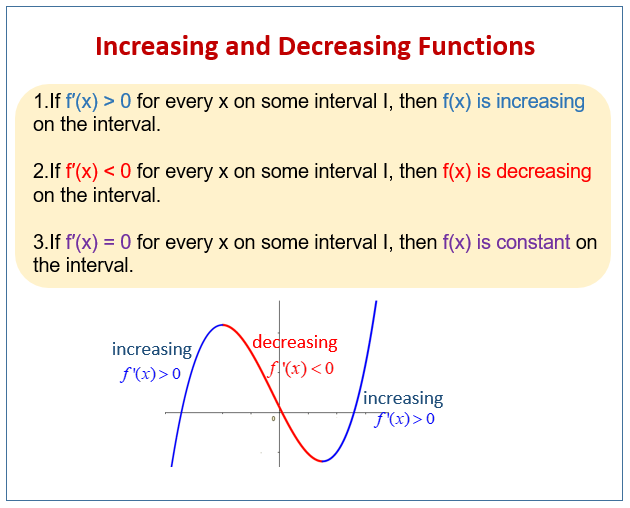
\includegraphics[scale=.75]{media/increasing-decreasing-functions.png}$$


\subsubsection{Concavity:}
$$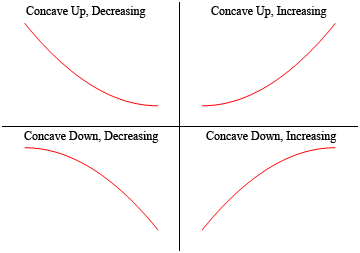
\includegraphics[scale=.75]{media/concavity.png}$$

\subsubsection{Extreme Value Theorem:} Suppose that $f(x)$ is continuous on the interval $[a,b]$ then there are two numbers, $a \leq c, d \leq d$ so that $f(c)$ is an absolute maximum for the function and $f(d)$ is an absolute minimum for the function.

\subsubsection{Fermat's Theorem:} If $f$ has a local max or min at $a$, and $f'(a)$ exists, then $f'(a) = 0$.

\subsubsection{Critical Number: } A critical number of a function $f$ is a number $c$ in the domain of $f$ such that either $f'(c) = 0$ or $f'(c) = $ DNE

\subsubsection{Absolute Extreme: } To find the absolute max and min values of a continuous function $f$ on a closed interval $[a,b]$: 

\begin{enumerate}
    \item Find the critical numbers of the function on $(a,b)$
    \item Find the values of $f$ at the critical numbers of $f$ in $(a,b)$
    \item Find the values of $f$ at the end points of the interval, in other words, find $f(a)$ and $f(b)$.
    \item The largest of the values from steps 2 and 3 is the absolute max, the smallest is the absolute min.
    
\end{enumerate}

\end{document}